%%%%%%%%%%%%%%%%%%%%%%%%%%%%%%%%%%%%%%%%%%%%%%%%%%%%%%%%%%%%%%%%%%%%%%
\section{\label{sec:GridUniverse}The Grid Universe}
%%%%%%%%%%%%%%%%%%%%%%%%%%%%%%%%%%%%%%%%%%%%%%%%%%%%%%%%%%%%%%%%%%%%%%

\index{Condor-C|(}

%%%%%%%%%%%%%%%%%%%%%%%%%%%%%%%%%%%%%%%%%%%%%%%%%%%%%%%%%%%%%%%%%%%%%%%%%%%
\subsection{\label{sec:Condor-C}Condor-C, The condor Grid Type }
%%%%%%%%%%%%%%%%%%%%%%%%%%%%%%%%%%%%%%%%%%%%%%%%%%%%%%%%%%%%%%%%%%%%%%%%%%%

\index{grid computing!Condor-C}
Condor-C allows jobs in one machine's job queue to
be moved to another machine's job queue.
These machines may be far removed from each other,
providing powerful grid computation mechanisms,
while requiring only Condor software and its configuration.

Condor-C is highly resistant to network disconnections and machine failures on both the submission and remote sides.
An expected usage
sets up Personal Condor on a laptop,
submits some jobs that are sent to a Condor pool,
waits until the jobs are staged on the pool,
then turns off the laptop.
When the laptop reconnects at a later time,
any results can be pulled back.

Condor-C scales gracefully when compared with Condor's flocking
mechanism.
The machine upon which jobs are submitted
maintains a single process and network connection to a remote machine,
without regard to the number
of jobs queued or running.

%%%%%%%%%%%%%%%%%%%%%%%%%%%%%%%%%%%%%%%%%%%%%%%%%%%%%%%%%%%%%%%%%%%%%%%%%%%
\subsubsection{\label{sec:Condor-C-Config}Condor-C Configuration}
%%%%%%%%%%%%%%%%%%%%%%%%%%%%%%%%%%%%%%%%%%%%%%%%%%%%%%%%%%%%%%%%%%%%%%%%%%%
\index{Condor-C!configuration}
There are two aspects to configuration to enable the
submission and execution of Condor-C jobs.
These two aspects correspond to the endpoints of the 
communication: there is the machine from which jobs are
submitted, and there is the remote machine upon which the
jobs are placed in the queue (executed).

Configuration of a machine from which jobs are submitted
requires a few extra configuration variables:

\footnotesize
\begin{verbatim}
CONDOR_GAHP=$(SBIN)/condor_c-gahp
C_GAHP_LOG=/tmp/CGAHPLog.$(USERNAME)
C_GAHP_WORKER_THREAD_LOG=/tmp/CGAHPWorkerLog.$(USERNAME)
\end{verbatim}
\normalsize

\index{Condor GAHP}
\index{GAHP (Grid ASCII Helper Protocol)}
The acronym GAHP stands for Grid ASCII Helper Protocol.
A GAHP server provides grid-related services for a
variety of underlying middle-ware systems.
The configuration variable \Macro{CONDOR\_GAHP}
gives a full path to the GAHP server utilized by Condor-C.
The configuration variable \Macro{C\_GAHP\_LOG} defines
the location of the log that the Condor GAHP server writes.
The log for the Condor GAHP is written as the user on whose
behalf it is running; thus the
\Macro{C\_GAHP\_LOG} configuration variable must point to a location the end
user can write to.

A submit machine must also have a \Condor{collector} daemon to which the
\Condor{schedd} daemon can submit a query.
The query is for the location (IP address and port)
of the intended remote machine's \Condor{schedd} daemon.
This facilitates communication between the two machines.
This \Condor{collector} does not need to be the same collector
that the local \Condor{schedd} daemon reports to.

The machine upon which jobs are executed 
must also be configured correctly.
This machine must be running a \Condor{schedd} daemon.
Unless specified explicitly in a submit file, 
\MacroNI{CONDOR\_HOST} must point to a 
\Condor{collector} daemon that it can write to,
and the machine upon which jobs are submitted can read from.
This facilitates communication between the two machines.

An important aspect of configuration is the security 
configuration relating to authentication.
Condor-C on the remote machine relies on an
authentication protocol to
know the identity of the user under which to run a job.
The following is a working example
of the security configuration for authentication.
This authentication method, CLAIMTOBE, 
trusts the identity claimed by a host or IP address.

\footnotesize
\begin{verbatim}
SEC_DEFAULT_NEGOTIATION = OPTIONAL
SEC_DEFAULT_AUTHENTICATION_METHODS = CLAIMTOBE
\end{verbatim}
\normalsize


%%%%%%%%%%%%%%%%%%%%%%%%%%%%%%%%%%%%%%%%%%%%%%%%%%%%%%%%%%%%%%%%%%%%%%%%%%%
\subsubsection{\label{sec:Condor-C-Submit}Condor-C Job Submission}
%%%%%%%%%%%%%%%%%%%%%%%%%%%%%%%%%%%%%%%%%%%%%%%%%%%%%%%%%%%%%%%%%%%%%%%%%%%
\index{Condor-C!job submission}
\index{universe!grid}
Job submission of Condor-C jobs is the same as for any Condor job.
The \SubmitCmd{universe} is \SubmitCmd{grid}.
\SubmitCmd{grid\_resource} specifies the remote \Condor{schedd} daemon to which
the job should be submitted, and its value consists of three fields.
The first field is the grid type, which is \SubmitCmd{condor}.
The second field is the name of the remote \Condor{schedd} daemon.
Its value is the
same as the \Condor{schedd} ClassAd attribute \Attr{Name} on the
remote machine.
The third field is the name of the remote pool's \Condor{collector}.
%and the \SubmitCmd{grid\_type} is \SubmitCmd{condor}. 
%The remote pool's job queue is defined and located by
%the submit description file command \SubmitCmd{remote\_schedd}.
%The value assigned for this command is the same as
%the \Condor{schedd} ClassAd attribute
%\Attr{Name} on the remote machine.
%The remote pool's \Condor{collector} is defined by the submit
%description file command \SubmitCmd{remote\_pool}.

The following represents a minimal submit description file for
a job.

\footnotesize
\begin{verbatim}
# minimal submit description file for a Condor-C job
universe = grid
executable = myjob
output = myoutput
error = myerror
log = mylog

grid_resource = condor joe@remotemachine.example.com remotecentralmanager.example.com
+remote_jobuniverse = 5
+remote_requirements = True
+remote_ShouldTransferFiles = "YES"
+remote_WhenToTransferOutput = "ON_EXIT"
queue
\end{verbatim}
\normalsize

The remote machine needs to understand the attributes of the job.
These are specified in the submit description file using the '+'
syntax, followed by the string \SubmitCmd{remote\_}.
At a minimum, this will be the job's \SubmitCmd{universe} and the job's
\SubmitCmd{requirements}.
It is likely that other attributes specific to the
job's \SubmitCmd{universe} (on the remote pool) will also be necessary.
Note that attributes set with '+' are inserted directly into
the job's ClassAd.  
Specify attributes as they 
must appear in the job's ClassAd, not the submit description file. 
For example,
the \SubmitCmd{universe} is specified using an integer assigned for
a job ClassAd \Attr{JobUniverse}.
Similarly, place quotation marks around string 
expressions.
As an example, a submit description file would ordinarily contain
\footnotesize
\begin{verbatim}
when_to_transfer_output = ON_EXIT
\end{verbatim}
\normalsize
This must appear in the Condor-C job submit description file as
\footnotesize
\begin{verbatim}
+remote_WhenToTransferOutput = "ON_EXIT"
\end{verbatim}
\normalsize

For convenience, the specific entries of 
\SubmitCmd{universe}, 
\SubmitCmd{remote\_grid\_resource}, 
\SubmitCmd{globus\_rsl}, and
\SubmitCmd{globus\_xml}
may be specified as \SubmitCmd{remote\_} commands
without the leading '+'. 
Instead of 
\footnotesize
\begin{verbatim}
+remote_universe = 5
\end{verbatim}
\normalsize

the submit description file command may appear as

\footnotesize
\begin{verbatim}
remote_universe = vanilla
\end{verbatim}
\normalsize

Similarly, the command
\footnotesize
\begin{verbatim}
+remote_gridresource = "condor schedd.example.com cm.example.com"
\end{verbatim}
\normalsize

may be given as

\footnotesize
\begin{verbatim}
remote_grid_resource = condor schedd.example.com cm.example.com
\end{verbatim}
\normalsize

% why we need +remote_ShouldTransferFiles, etc.
For the given example,
the job is to be run as a \SubmitCmd{vanilla} 
\SubmitCmd{universe} job at the remote pool.
The (remote pool's) \Condor{schedd} daemon is likely to
place its job queue data on a local disk 
and execute the job on another machine within the pool of machines.
This implies that the file systems for the resulting submit machine
(the machine specified by \SubmitCmd{remote\_schedd}) and
the execute machine (the machine that runs the job) will
\emph{not} be shared.
Thus,
the two inserted ClassAds
\footnotesize
\begin{verbatim}
+remote_ShouldTransferFiles = "YES"
+remote_WhenToTransferOutput = "ON_EXIT"
\end{verbatim}
\normalsize
are used to invoke Condor's file transfer mechanism. 



As Condor-C is a recent addition to Condor,
the universes, associated integer assignments,
and notes about the existence of functionality are given in 
Table~\ref{working-remote-universes}.
The note "untested" implies that
submissions under the given universe have not yet
been throughly tested.
They may already work.

% universes, and whether they work in Condor-C
% NEED TO UPDATE THIS TABLE FOR gt5 and cream
\begin{center}
\begin{table}[hbt]
\begin{tabular}{|l|l|l}
\textbf{Universe Name} & \textbf{Value} & \textbf{Notes}\\ \hline \hline
standard  & 1 & untested \\ \hline
vanilla   & 5 & works well \\ \hline
scheduler & 7 & works well \\ \hline
grid      & 9 & \\
 & grid\_resource is condor & works well \\
 & grid\_resource is cream & untested \\
 & grid\_resource is gt2  & works well \\
 & grid\_resource is gt4 & untested \\ 
 & grid\_resource is gt5 & untested \\ 
 & grid\_resource is nordugrid & untested \\ 
 & grid\_resource is unicore & untested \\
 & grid\_resource is lsf & works well \\
 & grid\_resource is pbs & works well \\ \hline
java & 10 & untested \\ \hline
parallel & 11 & untested \\ \hline
local & 12 & works well \\ \hline
\end{tabular}
\caption{\label{working-remote-universes}Functionality of remote job universes with Condor-C}
\end{table}
\end{center}

For communication between \Condor{schedd} daemons on the submit
and remote machines,
the location of the remote \Condor{schedd} daemon is needed.
This information resides in the \Condor{collector} of the remote
machine's pool.
The third field of the \SubmitCmd{grid\_resource} command in the submit description file
says which \Condor{collector} should be queried for the remote \Condor{schedd}
daemon's location.
An example of this submit command is
\footnotesize
\begin{verbatim}
grid_resource = condor schedd.example.com machine1.example.com
\end{verbatim}
\normalsize
If the remote \Condor{collector} is not listening on the standard port
(9618), then the port it \emph{is} listening on needs to be specified:
\footnotesize
\begin{verbatim}
grid_resource = condor schedd.example.comd machine1.example.com:12345
\end{verbatim}
\normalsize

File transfer of a job's executable, \File{stdin}, \File{stdout}, and
\File{stderr} are automatic.
When other files need to be transferred using Condor's file transfer
mechanism
(see section~\ref{sec:file-transfer} on page~\pageref{sec:file-transfer}),
the mechanism is applied based on the resulting job universe on the
remote machine.


%%%%%%%%%%%%%%%%%%%%%%%%%%%%%%%%%%%%%%%%%%%%%%%%%%%%%%%%%%%%%%%%%%%%%%%%%%%
\subsubsection{\label{sec:Condor-C-CrossPlatform}
Condor-C Jobs Between Differing Platforms}
%%%%%%%%%%%%%%%%%%%%%%%%%%%%%%%%%%%%%%%%%%%%%%%%%%%%%%%%%%%%%%%%%%%%%%%%%%%

Condor-C jobs given to a remote machine running Windows
must specify the Windows domain of the remote machine.
This is accomplished by defining a ClassAd attribute for the job.
Where the Windows domain is different at the submit machine
from the remote machine, the submit description file 
defines the Windows domain of the remote machine with
\begin{verbatim}
  +remote_NTDomain = "DomainAtRemoteMachine"
\end{verbatim}

A Windows machine not part of a domain
defines the Windows domain as the machine name.

%%%%%%%%%%%%%%%%%%%%%%%%%%%%%%%%%%%%%%%%%%%%%%%%%%%%%%%%%%%%%%%%%%%%%%%%%%%
%\subsubsection{\label{sec:Condor-C-Hops}Multiple Hops for Condor-C Jobs}
%%%%%%%%%%%%%%%%%%%%%%%%%%%%%%%%%%%%%%%%%%%%%%%%%%%%%%%%%%%%%%%%%%%%%%%%%%%
%
% \Todo

%%%%%%%%%%%%%%%%%%%%%%%%%%%%%%%%%%%%%%%%%%%%%%%%%%%%%%%%%%%%%%%%%%%%%%%%%%%
\subsubsection{\label{sec:Condor-C-Limits}Current Limitations in Condor-C}
%%%%%%%%%%%%%%%%%%%%%%%%%%%%%%%%%%%%%%%%%%%%%%%%%%%%%%%%%%%%%%%%%%%%%%%%%%%
\index{Condor-C!limitations}
Submitting jobs to run under the grid universe has not yet
been perfected.
The following is a list of known limitations with Condor-C:

\begin{enumerate}
  \item{Authentication methods other than
  \Expr{CLAIMTOBE}, such as \Expr{GSI} and \Expr{KERBEROS}, are 
  untested, and may not yet work.}

\end{enumerate}

\index{Condor-C|)}



\index{HTCondor-G|(}

%%%%%%%%%%%%%%%%%%%%%%%%%%%%%%%%%%%%%%%%%%%%%%%%%%%%%%%%%%%%%%%%%%%%%%%%%%%
\subsection{\label{sec:HTCondor-G}HTCondor-G, the gt2, and gt5 Grid Types}
%%%%%%%%%%%%%%%%%%%%%%%%%%%%%%%%%%%%%%%%%%%%%%%%%%%%%%%%%%%%%%%%%%%%%%%%%%%

HTCondor-G is the name given to HTCondor when \SubmitCmd{grid}
\SubmitCmd{universe} jobs are sent to grid resources utilizing
Globus software for job execution.
The Globus Toolkit provides a framework for building grid systems
and applications.
See the Globus Alliance web page at
\URL{http://www.globus.org}
for descriptions and details of the Globus software.

HTCondor provides the same job management capabilities for HTCondor-G
jobs as for other jobs.
From HTCondor, a user may effectively submit jobs, manage jobs,
and have jobs execute on widely distributed machines.

% HTCondor-G is a ``window to the grid.''
% The function of HTCondor-G becomes clear
% with a brief overview of the software that forms an HTCondor pool.
% For this discussion, the software of an HTCondor pool is divided
% into two parts.
% The first part does job management.
% It keeps track of a user's jobs.
% You can ask the job management part of HTCondor to show
% you the job queue, to submit new jobs to the system,
% to put jobs on hold,
% and to request information about jobs that have completed.
% The other part of the HTCondor software
% does resource management.
% It keeps track of which machines are available to run jobs,
% how the available machines should be utilized given all the users
% who want to run jobs on them,
% and when a machine is no longer available.
% HTCondor-G works with grid resources, allowing users to
% effectively submit jobs, manage jobs, and have jobs execute
% on widely distributed machines.

% A machine with the job management part installed
% is called a submit machine.
% A machine with the resource management part installed 
% is called an execute machine.
% Each machine may have one part or both.
% HTCondor-G is the job management part of HTCondor.
% \index{HTCondor-G!functionality}
% HTCondor-G lets you submit jobs into a queue,
% have a log detailing the life cycle of your jobs,
% manage your input and output files,
% along with everything else you expect from a job queuing system.

% HTCondor-G is a program that manages both a queue of jobs
% and the resources from one or more sites where those jobs can execute. 
% For some of these jobs,
% it communicates with these resources and transfers files
% to and from these resources using Globus mechanisms.
% (In particular, HTCondor-G uses the GRAM protocol for job submission,
% and it runs a local GASS server for file transfers).

It may appear that HTCondor-G is a simple replacement
for the Globus Toolkit's \Prog{globusrun} command.
However, HTCondor-G does much more.
It allows the submission of many jobs at once,
along with the monitoring of those jobs with a convenient interface.
There is notification when jobs complete or fail
and maintenance of Globus credentials
that may expire while a job is running.
On top of this, HTCondor-G is a fault-tolerant system;
if a machine crashes,
all of these functions are again available as the machine returns.



%%%%%%%%%%%%%%%%%%%%%%%%%%%%%%%%%%%%%%%%%%%%%%%%%%%%%%%%%%%%%%%%%%%%%%%%%%%
%%%%%%%%%%%%%%%%%%%%%%%%%%%%%%%%%%%%%%%%%%%%%%%%%%%%%%%%%%%%%%%%%%%%%%%%%%%
\subsubsection{\label{sec:Globus-Protocols}Globus Protocols and Terminology}
%%%%%%%%%%%%%%%%%%%%%%%%%%%%%%%%%%%%%%%%%%%%%%%%%%%%%%%%%%%%%%%%%%%%%%%%%%%
The Globus software provides a well-defined set of protocols
that allow authentication, data transfer, and remote job execution.
Authentication is a mechanism by which an identity is verified.
Given proper authentication, authorization to use a resource
is required.
Authorization is a policy that determines who is allowed to do what. 

HTCondor (and Globus) utilize the following protocols and terminology.
The protocols allow HTCondor to interact with grid machines toward
the end result of executing jobs.
\begin{description}
\item[GSI]
\index{GSI (Grid Security Infrastructure)}
The Globus Toolkit's Grid Security Infrastructure (GSI) provides essential
\index{HTCondor-G!GSI}
building blocks for other grid protocols and HTCondor-G.
This authentication and authorization system
makes it possible to authenticate a user just once,
using public key infrastructure (PKI) mechanisms to verify
a user-supplied grid credential.
GSI then handles the mapping of the grid credential to the
diverse local credentials and authentication/authorization mechanisms that
apply at each site. 
\item[GRAM]
The Grid Resource Allocation and Management (GRAM) protocol supports remote
\index{HTCondor-G!GRAM}
\index{GRAM (Grid Resource Allocation and Management)}
submission of a computational request (for example, to run a program)
to a remote computational resource,
and it supports subsequent monitoring and control of the computation. 
GRAM is the Globus protocol that HTCondor-G uses to talk to remote Globus
  jobmanagers.
\item[GASS]
The Globus Toolkit's Global Access to Secondary Storage (GASS) service provides
\index{HTCondor-G!GASS}
\index{GASS (Global Access to Secondary Storage)}
mechanisms for transferring data to and from a remote HTTP, FTP, or GASS server. 
GASS is used by HTCondor for the 
\SubmitCmd{gt2} grid type
to transfer a job's files
to and from the machine where the job is submitted and the remote resource.
\item[GridFTP]
GridFTP is an extension of FTP that provides strong security and 
high-performance options for large data transfers.
\item[RSL]
RSL (Resource Specification Language)  is the language GRAM 
accepts to specify job information.
\item[gatekeeper]
A gatekeeper is a software daemon executing on a remote machine on
the grid.
It is relevant only to the \SubmitCmd{gt2} grid type,
and this daemon handles the initial communication between
HTCondor and a remote resource.
\item[jobmanager]
A jobmanager is
the Globus service that is initiated at a remote resource to submit,
keep track of, and manage grid I/O for jobs running on 
an underlying batch system.
There is a specific jobmanager for each type of
batch system supported by Globus (examples are HTCondor, LSF, and PBS).

\end{description}


\begin{figure}[hbt]
\centering
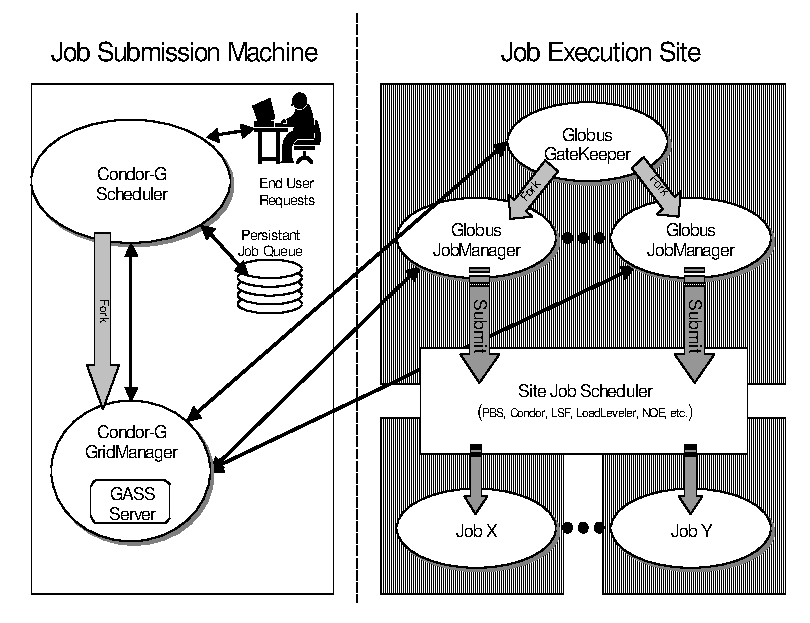
\includegraphics{grids/gfig1.eps}
\caption{\label{fig:condorg}HTCondor-G interaction with Globus-managed resources}
\end{figure}

Figure~\ref{fig:condorg} shows how HTCondor interacts with Globus software
towards running jobs.
The diagram is specific to the \SubmitCmd{gt2} type of grid.
HTCondor contains a GASS server, used to transfer the executable,
\File{stdin}, \File{stdout}, and \File{stderr} to and from
the remote job execution site.
HTCondor uses the GRAM protocol to contact the remote gatekeeper
and request that a new jobmanager be started.
The GRAM protocol is also used to when monitoring the job's progress.
HTCondor detects and intelligently handles cases
such as if the remote resource crashes.

There are now two different versions of the GRAM protocol in common
usage: \SubmitCmd{gt2} and \SubmitCmd{gt5}.
HTCondor supports both of them.
\begin{description}
\item[gt2]
This initial GRAM protocol is used in Globus Toolkit versions 1 and 2.
It is still used by many production systems.
Where available in the other, more recent versions of the protocol,
\SubmitCmd{gt2} is referred to as the pre-web services GRAM 
(or pre-WS GRAM) or GRAM2.

\item[gt5]
This latest GRAM protocol is an extension of GRAM2 that is intended to
be more scalable and robust. It's usually referred to as GRAM5.
\end{description}

%%%%%%%%%%%%%%%%%%%%%%%%%%%%%%%%%%%%%%%%%%%%%%%%%%%%%%%%%%%%%%%%%%%%%%%%%%%
\subsubsection{\label{sec:Using-gt2}The gt2 Grid Type}
%%%%%%%%%%%%%%%%%%%%%%%%%%%%%%%%%%%%%%%%%%%%%%%%%%%%%%%%%%%%%%%%%%%%%%%%%%%

\index{universe!grid, grid type gt2}
\index{grid computing!submitting jobs to gt2}
HTCondor-G supports submitting jobs to remote resources running
the Globus Toolkit's GRAM2 (or pre-WS GRAM) service. This flavor of GRAM
is the most common.
These HTCondor-G jobs are submitted the same as any other HTCondor job.
The \SubmitCmd{universe} is \SubmitCmd{grid},
and the pre-web services GRAM protocol is specified by
setting the type of grid as \SubmitCmd{gt2} in the \SubmitCmd{grid\_resource}
command.

\index{HTCondor-G!job submission}
\index{HTCondor-G!proxy}
\index{proxy}
Under HTCondor, successful job submission to the \SubmitCmd{grid} 
\SubmitCmd{universe} with \SubmitCmd{gt2}
requires credentials.
\index{HTCondor-G!X.509 certificate}
An X.509 certificate is used to create a proxy,
and an account, authorization, or allocation to use a grid resource
is required.
For general information on proxies and certificates,
please consult the Globus page at 

\URL{http://www-unix.globus.org/toolkit/docs/4.0/security/key-index.html}

Before submitting a job to HTCondor under the \SubmitCmd{grid} universe,
use \Prog{grid-proxy-init} to create a proxy.

Here is a simple submit description file.
\index{submit description file!grid universe}
The example specifies a \SubmitCmd{gt2} job to be run on
an NCSA machine.

\begin{verbatim}
executable = test
universe = grid
grid_resource = gt2 modi4.ncsa.uiuc.edu/jobmanager
output = test.out
log = test.log
queue
\end{verbatim} 

The 
\SubmitCmd{executable}
for this example is
transferred from the local machine to the remote machine.
By default, HTCondor transfers the executable, as well as any
files specified by an \SubmitCmd{input} command.
Note that the executable must be compiled for its intended platform.

\index{submit commands!grid\_resource}
The command \SubmitCmd{grid\_resource} is a required command
for grid universe jobs.
The second field specifies the scheduling software
to be used on the remote resource.
There is a specific jobmanager for each type of
batch system supported by Globus.
The full syntax for this command line appears as
\footnotesize
\begin{verbatim}
grid_resource = gt2 machinename[:port]/jobmanagername[:X.509 distinguished name]
\end{verbatim}
\normalsize
The portions of this syntax specification enclosed within
square brackets (\Lbr\ and \Rbr) are optional.
On a machine where the jobmanager is listening on a nonstandard port,
include the port number.
The \verb@jobmanagername@ is a site-specific string.
The most common one is \verb@jobmanager-fork@, but others are
\begin{verbatim}
jobmanager
jobmanager-condor
jobmanager-pbs
jobmanager-lsf
jobmanager-sge
\end{verbatim}
The Globus software running on the remote resource
uses this string to identify and select the correct service
to perform.
Other \verb@jobmanagername@ strings are used,
where additional services are defined and implemented.


The job log file is maintained on the submit machine.

Example output from 
\Condor{q} for this submission looks like:
\footnotesize
\begin{verbatim}
% condor_q


-- Submitter: wireless48.cs.wisc.edu : <128.105.48.148:33012> : wireless48.cs.wi

 ID      OWNER         SUBMITTED     RUN_TIME ST PRI SIZE CMD
   7.0   smith        3/26 14:08   0+00:00:00 I  0   0.0  test

1 jobs; 1 idle, 0 running, 0 held
\end{verbatim}
\normalsize

After a short time, the Globus resource accepts the job.
Again running \Condor{q} will now result in

\footnotesize
\begin{verbatim}
% condor_q


-- Submitter: wireless48.cs.wisc.edu : <128.105.48.148:33012> : wireless48.cs.wi

 ID      OWNER         SUBMITTED     RUN_TIME ST PRI SIZE CMD
   7.0   smith        3/26 14:08   0+00:01:15 R  0   0.0  test

1 jobs; 0 idle, 1 running, 0 held
\end{verbatim}
\normalsize

Then, very shortly after that, the queue will be empty again,
because the job has finished:

\footnotesize
\begin{verbatim}
% condor_q


-- Submitter: wireless48.cs.wisc.edu : <128.105.48.148:33012> : wireless48.cs.wi

 ID      OWNER            SUBMITTED     RUN_TIME ST PRI SIZE CMD

0 jobs; 0 idle, 0 running, 0 held
\end{verbatim}
\normalsize


A second example of a submit description file runs the Unix \Prog{ls}
program on a different Globus resource.

\footnotesize
\begin{verbatim}
executable = /bin/ls
transfer_executable = false
universe = grid
grid_resource = gt2 vulture.cs.wisc.edu/jobmanager
output = ls-test.out
log = ls-test.log
queue
\end{verbatim} 
\normalsize

In this example, the executable (the binary) has been pre-staged.
The executable is on the remote machine, and it is not to
be transferred before execution.
Note that the required 
\SubmitCmd{grid\_resource} and \SubmitCmd{universe}
commands are present.
The command
\begin{verbatim}
transfer_executable = false
\end{verbatim}
within the submit description file identifies the executable
as being pre-staged.
In this case, the 
\SubmitCmd{executable}
command gives the path to the executable on the remote machine.

A third example submits a Perl script to be run as a submitted
HTCondor job.
The Perl script both lists and sets
environment variables for a job.
Save the following Perl script with the name \File{env-test.pl},
to be used as an HTCondor job executable.

\begin{verbatim}
#!/usr/bin/env perl

foreach $key (sort keys(%ENV))
{
   print "$key = $ENV{$key}\n"
}

exit 0;
\end{verbatim}

Run the Unix command
\begin{verbatim}
chmod 755 env-test.pl
\end{verbatim}
to make the Perl script executable.

Now create the following submit description file.
Replace \File{example.cs.wisc.edu/jobmanager} with a resource
you are authorized to use.

\footnotesize
\begin{verbatim}
executable = env-test.pl
universe = grid
grid_resource = gt2 example.cs.wisc.edu/jobmanager
environment = foo=bar; zot=qux
output = env-test.out
log = env-test.log
queue
\end{verbatim}
\normalsize

When the job has completed, the output file, \File{env-test.out},
should contain something like this:

\footnotesize
\begin{verbatim}
GLOBUS_GRAM_JOB_CONTACT = https://example.cs.wisc.edu:36213/30905/1020633947/
GLOBUS_GRAM_MYJOB_CONTACT = URLx-nexus://example.cs.wisc.edu:36214
GLOBUS_LOCATION = /usr/local/globus
GLOBUS_REMOTE_IO_URL = /home/smith/.globus/.gass_cache/globus_gass_cache_1020633948
HOME = /home/smith
LANG = en_US
LOGNAME = smith
X509_USER_PROXY = /home/smith/.globus/.gass_cache/globus_gass_cache_1020633951
foo = bar
zot = qux
\end{verbatim}
\normalsize


Of particular interest is the \Env{GLOBUS\_REMOTE\_IO\_URL}
environment variable.
HTCondor-G automatically starts up a GASS remote I/O
server on the submit machine.
Because of the potential for either side of the connection to fail,
the URL for the server cannot be passed directly to the job.
Instead, it is placed into a file, and the \Env{GLOBUS\_REMOTE\_IO\_URL}
environment variable points to this file.
Remote jobs can read this file and use the URL it contains
to access the remote GASS server running inside HTCondor-G.
If the location
of the GASS server changes (for example, if HTCondor-G restarts),
HTCondor-G will contact the Globus gatekeeper and update this file on
the machine where the job is running.
It is therefore important that all accesses to
the remote GASS server check this file for the latest location.

The following example is a Perl script that uses the GASS server in HTCondor-G
to copy input files to the execute machine.
In this example, the remote job
counts the number of lines in a file.

\footnotesize
\begin{verbatim}
#!/usr/bin/env perl
use FileHandle;
use Cwd;

STDOUT->autoflush();
$gassUrl = `cat $ENV{GLOBUS_REMOTE_IO_URL}`;
chomp $gassUrl;

$ENV{LD_LIBRARY_PATH} = $ENV{GLOBUS_LOCATION}. "/lib";
$urlCopy = $ENV{GLOBUS_LOCATION}."/bin/globus-url-copy";

# globus-url-copy needs a full path name
$pwd = getcwd();
print "$urlCopy $gassUrl/etc/hosts file://$pwd/temporary.hosts\n\n";
`$urlCopy $gassUrl/etc/hosts file://$pwd/temporary.hosts`;

open(file, "temporary.hosts");
while(<file>) {
print $_;
}

exit 0;
\end{verbatim}
\normalsize

The submit description file used to submit the Perl script as
an HTCondor job appears as:

\footnotesize
\begin{verbatim}
executable = gass-example.pl
universe = grid
grid_resource = gt2 example.cs.wisc.edu/jobmanager
output = gass.out
log = gass.log
queue
\end{verbatim}
\normalsize

There are two optional submit description file commands
of note:
\SubmitCmd{x509userproxy} and
\SubmitCmd{globus\_rsl}.
The \SubmitCmd{x509userproxy} command specifies the path to
an X.509 proxy.
The command is of the form:
\begin{verbatim}
x509userproxy = /path/to/proxy
\end{verbatim}
If this optional command is not present in the submit description file,
then HTCondor-G checks the value of the environment variable
\Env{X509\_USER\_PROXY} for the location of the proxy.
If this environment variable is not present, then HTCondor-G
looks for the proxy in the file
\File{/tmp/x509up\_uXXXX},
where the characters \verb@XXXX@ in this file name are
replaced with the Unix user id.

The \SubmitCmd{globus\_rsl} command is used to add additional
attribute settings to a job's RSL string.
The format of the \SubmitCmd{globus\_rsl} command is
\begin{verbatim}
globus_rsl = (name=value)(name=value)
\end{verbatim}
Here is an example of this command from a submit description file:
\begin{verbatim}
globus_rsl = (project=Test_Project)
\end{verbatim}
This example's attribute name for the additional RSL is
\AdAttr{project}, and the value assigned is \AdAttr{Test\_Project}.


%%%%%%%%%%%%%%%%%%%%%%%%%%%%%%%%%%%%%%%%%%%%%%%%%%%%%%%%%%%%%%%%%%%%%%%%%%%
\subsubsection{\label{sec:Using-gt5}The gt5 Grid Type}
%%%%%%%%%%%%%%%%%%%%%%%%%%%%%%%%%%%%%%%%%%%%%%%%%%%%%%%%%%%%%%%%%%%%%%%%%%%

\index{universe!grid, grid type gt5}
\index{grid computing!submitting jobs to gt5}

The Globus GRAM5 protocol works the same as the gt2 grid type.
Its implementation differs from gt2 in the following 3 items:
\begin{itemize}
\item
The Grid Monitor is disabled.
\item
Globus job managers are not stopped and restarted. 
\item
The configuration variable \Macro{GRIDMANAGER\_MAX\_JOBMANAGERS\_PER\_RESOURCE} 
is not applied (for gt5 jobs).
\end{itemize}

Normally, HTCondor will automatically detect whether a service is GRAM2 or
GRAM5 and interact with it accordingly. 
It does not matter whether gt2 or gt5 is specified. 
Disable this detection by setting
the configuration variable \Macro{GRAM\_VERSION\_DETECTION} to \Expr{False}.
If disabled, each resource must be accurately identified as either gt2 or gt5
in the \SubmitCmd{grid\_resource} submit command.

%%%%%%%%%%%%%%%%%%%%%%%%%%%%%%%%%%%%%%%%%%%%%%%%%%%%%%%%%%%%%%%%%%%%%%%%%%%
\subsubsection{\label{sec:My-Proxy}Credential Management with \Prog{MyProxy}}
%%%%%%%%%%%%%%%%%%%%%%%%%%%%%%%%%%%%%%%%%%%%%%%%%%%%%%%%%%%%%%%%%%%%%%%%%%%
\index{proxy!renewal with \Prog{MyProxy}}
HTCondor-G can use \Prog{MyProxy}
software to automatically renew GSI proxies for
\SubmitCmd{grid}
\SubmitCmd{universe} jobs with grid type
\SubmitCmd{gt2}.
\Prog{MyProxy} is a software component developed at
NCSA and used widely throughout the grid community.
For more information see:
\URL{http://myproxy.ncsa.uiuc.edu/}

Difficulties with proxy expiration occur in two cases.
The first case are long running jobs, which do not complete
before the proxy expires.
The second case occurs when great numbers of jobs are submitted.
Some of the jobs may not yet be started
or not yet completed before the proxy expires.
One proposed solution to these difficulties is to generate
longer-lived proxies.
This, however, presents a greater security problem.
Remember that a GSI proxy is sent to the remote Globus resource.
If a proxy falls into the hands of a malicious user at the remote site,
the malicious user can impersonate the proxy owner
for the duration of the proxy's lifetime.
The longer the proxy's lifetime,
the more time a malicious user has to misuse the owner's credentials.
To minimize the
window of opportunity of a
malicious user, 
it is recommended that proxies have a short lifetime
(on the order of several hours).

The \Prog{MyProxy} software generates proxies using credentials
(a user certificate or a long-lived proxy) located on a secure
\Prog{MyProxy} server.
HTCondor-G talks to the MyProxy server,
renewing a proxy as it is about to expire.
Another advantage that this presents is it relieves the user
from having to store a GSI user certificate and private key
on the machine where jobs are submitted.
This may be particularly important if a shared HTCondor-G
submit machine is used by several users.

In the a typical case, the following steps occur:

\begin{enumerate}
\item{The user creates a long-lived credential}
on a secure \Prog{MyProxy} server, using the
\Prog{myproxy-init} command.
Each organization generally has their own \Prog{MyProxy} server.

\item{The user creates a short-lived proxy}
on a local submit machine,
using
\Prog{grid-proxy-init} or \Prog{myproxy-get-delegation}.

\item{The user submits}
an HTCondor-G job,
specifying:
\begin{description}
\item{\Prog{MyProxy} server name (host:port)}
\item{\Prog{MyProxy} credential name (optional)}
\item{\Prog{MyProxy} password}
\end{description}

\item{At the short-lived proxy expiration}
HTCondor-G talks to
the \Prog{MyProxy} server to refresh the proxy.

\end{enumerate}


HTCondor-G keeps track of the password to the \Prog{MyProxy} server
for credential renewal.
Although HTCondor-G tries to keep the password encrypted and secure,
it is still possible (although highly unlikely) for the password
to be intercepted from the HTCondor-G machine
(more precisely, from the machine that the
\Condor{schedd} daemon that manages the grid universe jobs runs on,
which may be distinct from the machine from where jobs are submitted).
The following safeguard practices are recommended.

\begin{enumerate}

\item{Provide time limits}
for credentials on the \Prog{MyProxy} server.
The default is one week, but you may want to make it shorter.
%(See --cred_lifetime option to myproxy-init).

\item{Create several different \Prog{MyProxy} credentials},
maybe as many as one for each submitted job.
Each credential has a unique name,
which is identified with the
\Attr{MyProxyCredentialName} command in the submit description file.

\item{Use the following options}
when initializing the credential on the \Prog{MyProxy} server:

\footnotesize
\begin{verbatim}
myproxy-init -s <host> -x -r <cert subject> -k <cred name>
\end{verbatim}
\normalsize

The option \OptArg{-x -r}{<cert subject>}
essentially tells the \Prog{MyProxy} server to require two forms
of authentication:
  \begin{enumerate}
  \item{a password (initially set with \Prog{myproxy-init})}
  \item{an existing proxy (the proxy to be renewed)}
  \end{enumerate}

\item{A submit description file may include the password.}
An example contains commands of the form:
\footnotesize
\begin{verbatim}
executable      = /usr/bin/my-executable
universe        = grid
grid_resource   = gt2 condor-unsup-7
MyProxyHost     = example.cs.wisc.edu:7512
MyProxyServerDN = /O=doesciencegrid.org/OU=People/CN=Jane Doe 25900
MyProxyPassword = password
MyProxyCredentialName = my_executable_run
queue
\end{verbatim}
\normalsize
Note that placing the password within the submit file
is not really secure,
as it relies upon whatever file system security there is.
This may still be better than option 5.

\item{Use the \Opt{-p} option to \Condor{submit}.}
The submit command appears as
\footnotesize
\begin{verbatim}
condor_submit -p mypassword /home/user/myjob.submit
\end{verbatim}
\normalsize
The argument list for \Condor{submit} defaults to
being publicly available.
An attacker with a log in to the local machine could
generate a simple shell script
%  such as:
%  while 1; ps -efwww| grep 'condor_submit.*-p';done
to watch for the password. 

\end{enumerate}

Currently, HTCondor-G calls the
\Prog{myproxy-get-delegation} command-line tool,
passing it the necessary arguments.
The location of the
\Prog{myproxy-get-delegation} executable is determined by the
configuration variable
\Macro{MYPROXY\_GET\_DELEGATION} in the configuration file
on the HTCondor-G machine.
This variable is read by the \Condor{gridmanager}.
If
\Prog{myproxy-get-delegation}
is a dynamically-linked executable
(verify this with \Code{ldd myproxy-get-delegation}),
point
\MacroNI{MYPROXY\_GET\_DELEGATION}
to a wrapper shell script that sets
\MacroNI{LD\_LIBRARY\_PATH} to the correct \Prog{MyProxy}
library or Globus library directory and then
calls \Prog{myproxy-get-delegation}.
Here is an example of such a wrapper script:

\footnotesize
\begin{verbatim}
#!/bin/sh
export LD_LIBRARY_PATH=/opt/myglobus/lib
exec /opt/myglobus/bin/myproxy-get-delegation $@
\end{verbatim}
\normalsize


%%%%%%%%%%%%%%%%%%%%%%%%%%%%%%%%%%%%%%%%%%%%%%%%%%
\subsubsection{\label{sec:Condor-G-GridMonitor}The Grid Monitor}
%%%%%%%%%%%%%%%%%%%%%%%%%%%%%%%%%%%%%%%%%%%%%%%%%%
\index{Grid Monitor}
\index{grid computing!Grid Monitor}
\index{scalability!using the Grid Monitor}

Condor's Grid Monitor is designed to improve the scalability of
machines running the Globus Toolkit's GRAM2 gatekeeper.
Normally, this service runs a jobmanager process for 
every job submitted to the gatekeeper.
This includes both currently running jobs and jobs waiting in the queue.
Each jobmanager runs a Perl script at
frequent intervals (every 10 seconds) to poll the state of
its job in the local batch system.
For example, with 400 jobs submitted to a gatekeeper,
there will be 400 jobmanagers running,
each regularly starting a Perl script.
When a large number of jobs
have been submitted to a single gatekeeper,
this frequent polling can heavily load the gatekeeper.
When the gatekeeper is under heavy load,
the system can become non-responsive, and a variety of problems can occur.

Condor's Grid Monitor temporarily replaces these jobmanagers.
It is named the Grid Monitor, because it replaces the monitoring
(polling) duties previously done by jobmanagers.
When the Grid Monitor runs,
Condor attempts to start a single
process to poll all of a user's jobs at a given gatekeeper.
While a job is waiting in the queue, but not yet running,
Condor shuts down the associated jobmanager,
and instead relies on the Grid Monitor to report changes in status.
The jobmanager started to add the job to the remote
batch system queue is shut down.
The jobmanager restarts when the job begins running.

The Grid Monitor requires that the gatekeeper support the fork
jobmanager with the name \Prog{jobmanager-fork}.
If the gatekeeper does not support the fork jobmanager,
the Grid Monitor will not be used for that site.
The \Condor{gridmanager} log file reports any problems
using the Grid Monitor.

The Grid Monitor is enabled by default,
and the
configuration macro \Macro{GRID\_MONITOR} identifies
the location of the executable.


%%%%%%%%%%%%%%%%%%%%%%%%%%%%%%%%%%%%%%%%%%%%%%%%%%%%%%%%%%%%%%%%%%%%%%%%%%%





%%%%%%%%%%%%%%%%%%%%%%%%%%%%%%%%%%%%%%%%%%%%%%%%%%%%%%%%%%%%%%%%%%%%%%%%%%%
\subsubsection{\label{sec:HTCondor-G-Limits}Limitations of HTCondor-G}
%%%%%%%%%%%%%%%%%%%%%%%%%%%%%%%%%%%%%%%%%%%%%%%%%%%%%%%%%%%%%%%%%%%%%%%%%%%
% This subsubsection used to reside in the file limitations.tex.
\index{HTCondor-G!limitations}
Submitting jobs to run under the grid universe has not yet
been perfected.
The following is a list of known limitations:

\begin{enumerate}
\item{No checkpoints.}
\item{No job exit codes.}
Job exit codes are not available when using
\SubmitCmd{gt2}.
\item{Limited platform availability.}
Windows support is not yet available.
\end{enumerate}

\index{HTCondor-G|)}




This section contains information relevant to all grid-types. The 
following sections contain information specific to particular grid-types.

%%%%%%%%%%%%%%%%%%%%%%%%%%%%%%%%%%%%%%%%%%%%%%%%%%%%%%%%%%%%%%%%%%%%%%%%%%%
\subsection{Removing Grid Universe jobs}
%%%%%%%%%%%%%%%%%%%%%%%%%%%%%%%%%%%%%%%%%%%%%%%%%%%%%%%%%%%%%%%%%%%%%%%%%%%

When you remove a job with \Condor{rm}, you may find that the job
enters the ``X'' state for a very long time. This is normal: Condor
is attempting to communicate with the remote scheduling system and
ensure that the job has been properly cleaned up. If it takes too long
or (in rare circumstances) is never removed, you can force the job to
leave the job queue by using the -forcex option to \Condor{rm}. This
will forcibly remove jobs that are in the X state without attempting
to finish any cleanup at the remote scheduler.


%subsection on matchmaking in the grid universe
%%%%%%%%%%%%%%%%%%%%%%%%%%%%%%%%%%%%%%%%%%%%%%%%%%
\subsection{\label{sec:Condor-G-Matchmaking}Condor-G-Matchmaking}
%%%%%%%%%%%%%%%%%%%%%%%%%%%%%%%%%%%%%%%%%%%%%%%%%%
\index{universe!Globus}
\index{Globus}
\index{matchmaking!Grid}

In it simplest usage, Condor-G allows users to specify exactly which
grid site they wish to submit their job to. Often this is
sufficient: perhaps a user knows exactly which grid site they wish to
use, or a higher-level resource broker (such as the European Data
Grid's resource broker) has decided which grid site should be
used. But when users have a variety of sites to choose from and there
is no other resource broker to make the decision, Condor-G can use
matchmaking to decide which grid site a job should run on. 

Please note that Condor-G's matchmaking ability is relatively
new. Work is being done to improve it and make it easier to use. For
now, please expect some rough edges. 

Condor-G uses the same matchmaking mechanism that Condor uses: the
Condor collector and negotiator, which are described in
Section~\ref{sec:Condor-Daemons}. 

To use Condor-G's matchmaking, you need to make two changes. First,
you need to advertise grid sites that are available so that they are
known during the matchmaking process. Second, the submit file that
describes the job needs to specify requirements that describe what
type of grid site can be instead of specifying a specific grid site.

%%%%%%%%%%%%%%%%%%%%%%%%%%%%%%%%%%%%%%%%%%%%%%%%%%
\subsubsection{Advertising grid sites to Condor-G}
%%%%%%%%%%%%%%%%%%%%%%%%%%%%%%%%%%%%%%%%%%%%%%%%%%

Each grid site that is available for matching purposes needs to be
advertisted to the \Condor{collector}. Normally in Condor this is done
with the \Condor{startd} daemon, and you do not normally need to be
aware of the contents of this advertisement. Currently, there is no
equivalent to the \Condor{startd} daemon for advertising grid sites,
so you need have a deeper understanding. 

To properly advertise a grid site, a ClassAd need to be sent
periodically to the \Condor{collector}. A ClassAd is a list of
attributes and values that describe a job, a machine, or a grid
site. ClassAds are briefly described in
Section~\ref{sec:matchmaking-with-classads} and some of the common
attributes of machine ClassAds are described in
Section~\ref{user-man-machad}.

When you advertise a grid site, it looks very similar to a ClassAd for
a machine. In fact, the \Condor{collector} will believe it is a
machine, but with a different set of attributes. 

To advertise a grid site, you first need to describe the site in a
file. Here is a sample ClassAd that describes a grid site:

\begin{verbatim}
# This is a comment
MyType                = "Machine"
TargetType            = "Job"
Name                  = "Example1_Gatekeeper"
gatekeeper_url        = "grid.example.com/jobmanager"
Requirements          = CurMatches < 10
Rank                  = 0.000000
CurrentRank           = 0.000000
WantAdRevaluate       = True
UpdateSequenceNumber  = 4
CurMatches            = 0
\end{verbatim}

Let's look at each line:

\begin{verbatim}
# This is a comment
\end{verbatim}

Your file can have comments that begin with the hash mark (\#). 

\begin{verbatim}
MyType                = "Machine"
\end{verbatim}

Your grid site is pretending to be a single machine, for the purpose
of matchmaking. MyType is an attribute that the \Condor{negotiator}
will expect to be a string. Strings must be surrounded by double-quote
marks, as in this example. You may have surprising, unintuitive errors
if they are not quoted. You will always want MyType to be
``Machine''. 

\begin{verbatim}
TargetType            = "Job"
\end{verbatim}

This is an attribute that says the grid site (machine) wants to be
matched with a job. Leave this as it is. 


\begin{verbatim}
Name                  = "Example1_Gatekeeper"
\end{verbatim}

You will want a unique name for each grid site. Any name is fine, as long as
it is quoted.

\begin{verbatim}
gatekeeper_url        = "grid.example.com/jobmanager"
\end{verbatim}

This is the Globus gatekeeper contact string for your grid site. It is
probably a machine name followed by a slash followed by the name of
the jobmanager. If you have different job managers, you can only
specify one per ClassAd. 

\begin{verbatim}
UpdateSequenceNumber  = 4
\end{verbatim}

UpdateSequenceNumber is a positive number that must increase each time
you advertise a grid site. Normally you advertise your grid site
every five minutes. The \Condor{collector} will discard a grid site's
ClassAd after 15 minutes if there have been no updates. A good number
to set this to is the current time in seconds (the epoch, as given by
the C time() function call), but if you are worried about your clock
running backward, you can set it to whatever you like. If ClassAds are
received with a sequence number older than the last ClassAd, they are
ignored. 

\begin{verbatim}
CurMatches            = 0
\end{verbatim}

This number is incremented each time a match is made for this grid
site. Unlike a normal machine ClassAd that can only be matched against
once, grid site advertisements can be matched against many time. 

You will probably want to set this number to be the number of grid
jobs that you have running on your site, and keep it updated each time
you submit a new ClassAd. If you do not specify CurMatches, Condor
will assume it is 0.

Condor will increment this number every time it makes a match against
a grid site.

\begin{verbatim}
Requirements          = CurMatches < 10
\end{verbatim}

These are the requirements that the grid site insists must be trust
before it will accept a job. These could refer to features of the
job's ClassAd. In this case, we'll take any job, as long we have less
than 10 matches currently. This will ensure that Condor-G will only
run 10 jobs at your site---assuming that you keep CurMatches up to
date when jobs finish. Of course, you can edit this statement to have
different requirements. For example, if you want to accept all jobs,
you can have ``Requirements = True''. 

\begin{verbatim}
Rank                  = 0.000000
CurrentRank           = 0.000000
\end{verbatim}

This is a numerical ranking that will be assigned to a job. Right now
it is not used, but should be set to 0. 

\begin{verbatim}
WantAdRevaluate       = True
\end{verbatim}

This should be in your ad and should be true. Note that True is not in
quotes, and it should not be. This is what distinguishes grid site
ClassAds from normal machine ClassAds and allows multiple matches to
be made against a single site. 

You can add other attributes to your ClassAd, to make it easy for a
job to decide which grid site it wants to use. For instance, if you
have pre-installed the Bamboozle software environment on your grid
site, you could advertise, ``HaveBamboozle = True'' and
``BamboozleVersion = 10''. Jobs can require a grid site that has
Bamboozle installed by extending their requirements with
``HaveBamboozle == True''. (Note the double equal sign in the
requirements.) 

As an aside, we recommend that jobs that need specific applications
should bring them with them instead of relying on having them
pre-installed at a Grid site. You will have more reliable execution if
you do. 

Once you have a file that describes your site, you need to send it to
the \Condor{collector}. For this, you can use the \Condor{advertise}
program. We recommend that you write a script to create the file
containing the ClassAd, then run the script every five minutes with
cron. The script should probably update the CurMatches variable if you
want to restict the number of grid jobs that can be submitted at one
time. 

For \Condor{advertise} you will need to specify UPDATE\_STARTD\_AD for
the update command. For example, if your ClassAd is specified in a
file named ``grid-ad'' you would do:

\begin{verbatim}
    condor_advertise UPDATE_STARTD_AD grid-ad
\end{verbatim}

\Condor{advertise} usually uses UDP to transmit your ClassAd. In
wide-area networks, this may be insufficient. You can use TCP by
specifying the ``-tcp'' option. 

%%%%%%%%%%%%%%%%%%%%%%%%%%%%%%%%%%%%%%%%%%%%%%%%%%
\subsubsection{Submitting Condor-G jobs that use matchmaking}
%%%%%%%%%%%%%%%%%%%%%%%%%%%%%%%%%%%%%%%%%%%%%%%%%%

Submitting a job to Condor-G that requires matchmaking is
straightforward. Instead of specifying a particular scheduler with
globussheduler like this:

\begin{verbatim}
globusscheduler = grid.example.com/jobmanager
\end{verbatim}

you instead specify requirements and tell Condor-G where to find the
gatekeeper URL in the grid site ClassAd:

\begin{verbatim}
globusscheduler = $$(gatekeeper_url)
requirements    = true
\end{verbatim}

This will allow to run at any grid site, and will extract the
gatekeeper\_url attribute from the ClassAd. There is no magic meaning
behind gatekeeper\_url---you could use GatekeeperContactString if you
desired, as long as it is the same in both the job description and the
grid site ClassAd. 

The requirements specified here are a bit simple. Perhaps you only
want to run at a site that has the Bamboozle software installed, and
the sites that have it installed specify ``HaveBamboozle = True'', as
described above. A complete job description may look like this:

\begin{verbatim}
universe        = globus
executable      = analyze_bamboozle_data
output          = aaa.$(Cluster).out
error           = aaa.$(Cluster).err
log             = aaa.log
globusscheduler = $$(gatekeeper_url)
leave_in_queue  = jobstatus == 4
queue
\end{verbatim}

%%%%%%%%%%%%%%%%%%%%%%%%%%%%%%%%%%%%%%%%%%%%%%%%%%
\subsubsection{Advanced usage}
%%%%%%%%%%%%%%%%%%%%%%%%%%%%%%%%%%%%%%%%%%%%%%%%%%

What if a job fails to run at a grid site due to an error? It will be
returned to the queue, and Condor will attempt to match it and
re-run it at another site. Condor isn't very clever about avoiding
sites that may be bad, but you can give it some assistance. Let's say
that you want to avoid running at the last grid site you ran at. You
could add this to your job description:

\begin{verbatim}
match_list_length = 1
Rank              = TARGET.Name != LastMatchName0
\end{verbatim}

This will prefer to run at a grid site that was not just tried, but it
will allow the job to be run there if there is no other option. 

When you specify match\_list\_length, you provide an integer N, and
Condor will keep track of the last N matches. The oldest match will be
LastMatchName0, and next oldest will be LastMachName1, and so on. (See
the \Condor{submit} manual page for more details.) The Rank expression
allows you to specify a numerical ranking for different matches. When
combined with match\_list\_length, you can prefer to avoid sites that
you have already run at. 

In addition, \Condor{submit} has two options to help you control
Condor-G job resubmissions and rematching. See globus\_resubmit and
globus\_rematch in the \Condor{submit} manual page. 

There are some new attributes that will be added to the Job ClassAd,
and may be useful to you when you write your rank, requirements,
globus\_resubmit or globus\_rematch option. Please refer to
Section~\ref{user-man-jobad} and read about the following option:

\begin{itemize}
\item NumJobMatches
\item NumGlobusSubmits
\item NumSystemHolds
\item HoldReason
\item ReleaseReason
\item EnteredCurrentStatus
\item LastMatchTime
\item LastRejMatchTime
\item LastRejMatchReason
\end{itemize}

If you are concerned about unknown or malicious grid sites reporting
to your \Condor{collector}, you should use Condor's security options,
documented in Section~\ref{sec:Security}.

